\documentclass[12pt,a4paper]{report}
\usepackage[romanian]{babel}
\usepackage[utf8]{inputenc}
\usepackage[T1]{fontenc}
\usepackage{times}
\usepackage[left=3cm,right=2cm,top=2cm,bottom=2cm]{geometry}
\usepackage{setspace}
\onehalfspacing
\usepackage{graphicx}
\usepackage{float}
\usepackage{array}
\usepackage{tabularx}
\usepackage{booktabs}
\usepackage{url}
\usepackage{hyperref}
\usepackage{fancyhdr}
\usepackage{lastpage}
\usepackage{courier}
\usepackage{listings}
\usepackage{xcolor}
\usepackage{caption}
\usepackage{subcaption}
\usepackage{amssymb}
\usepackage{indentfirst}
\usepackage[bottom]{footmisc}
\usepackage{tikz}
\usepackage[utf8]{inputenc}
\usepackage[romanian]{babel}
\usetikzlibrary{shapes,arrows,positioning,shadows}
\setlength{\footnotesep}{0.7\baselineskip}
\renewcommand{\footnoterule}{\vfill\kern-3pt\hrule width 0.4\columnwidth\kern2.6pt}
% Configurare pentru listinguri de cod
\lstset{
    basicstyle=\footnotesize\ttfamily,
    numbers=left,
    numberstyle=\tiny,
    stepnumber=1,
    numbersep=5pt,
    backgroundcolor=\color{gray!10},
    showspaces=false,
    showstringspaces=false,
    showtabs=false,
    frame=single,
    rulecolor=\color{black},
    tabsize=2,
    captionpos=b,
    breaklines=true,
    breakatwhitespace=false,
    title=\lstname,
}

% Configurare headers și footers
\pagestyle{fancy}
\fancyhf{}
\fancyfoot[C]{\thepage}
\renewcommand{\headrulewidth}{0pt}
\renewcommand{\footrulewidth}{0pt}
\setlength{\headheight}{14.5pt}  % Fix fancyhdr warning

% Justificare text
\usepackage{ragged2e}
\justifying

\begin{document}

% COPERTA
\begin{titlepage}
\begin{center}
\large
UNIVERSITATEA „ALEXANDRU IOAN CUZA" DIN IAȘI\\
\vspace{0.5cm}
\textbf{FACULTATEA DE INFORMATICĂ}\\
\vspace{2cm}


\includegraphics[width=4cm]{logo_uaic.png}\\
\vspace{2cm}

\Large
\textbf{LUCRARE DE LICENȚĂ}\\
\vspace{1.5cm}

\huge
\textbf{CivicAlert: Platformă Web Interactivă\\pentru Raportarea Problemelor Civice}\\
\vspace{1cm}

\large
propusă de\\
\vspace{0.5cm}
\textbf{Prenume Nume}\\
\vspace{2cm}

\textbf{Sesiunea:} iunie, anul\\
\vspace{1cm}

\textbf{Coordonator științific}\\
\textbf{Titlu Prenume Nume}\\

\end{center}
\end{titlepage}

% PAGINA DE TITLU
\newpage
\begin{center}
\large
UNIVERSITATEA „ALEXANDRU IOAN CUZA" DIN IAȘI\\
\vspace{0.5cm}
\textbf{FACULTATEA DE INFORMATICĂ}\\
\vspace{4cm}

\huge
\textbf{CivicAlert: Platformă Web Interactivă\\pentru Raportarea Problemelor Civice}\\
\vspace{2cm}

\large
\textbf{Prenume Nume}\\
\vspace{2cm}

\textbf{Sesiunea:} iunie, anul\\
\vspace{4cm}

\textbf{Coordonator științific}\\
\textbf{Titlu Prenume Nume}\\

\end{center}

% DECLARAȚIA DE ORIGINALITATE
\newpage
\begin{flushright}
\textbf{Avizat,}\\
Îndrumător Lucrare de Licență\\
Titlu, Numele și prenumele \makebox[6cm]{\dotfill}\\
Data \makebox[2cm]{\dotfill} Semnătura \makebox[3cm]{\dotfill}\\
\end{flushright}

\vspace{2cm}

\textbf{DECLARAȚIE privind originalitatea conținutului lucrării de licență}

\vspace{1cm}

Subsemnatul(a) \dotfill\\
domiciliul \dotfill în \dotfill\\
\dotfill născut(ă) la data de \ldots\ldots\ldots\ldots\ldots, identificat prin CNP \ldots\ldots\ldots\ldots\ldots\ldots\ldots\ldots\ldots\ldots, absolvent(a) al(a) Universității „Alexandru Ioan Cuza" din Iași, Facultatea de \ldots\ldots\ldots\ldots specializarea \ldots\ldots\ldots\ldots\ldots\ldots, promovată \ldots\ldots\ldots\ldots, declar pe propria răspundere, cunoscând consecințele falsului în declarații în sensul art. 326 din Noul Cod Penal și dispozițiile Legii Educației Naționale nr. 1/2011 art.143 al. 4 și 5 referitoare la plagiat, că lucrarea de licență cu titlul:\\
\ldots\ldots\ldots\ldots\ldots\ldots\ldots\ldots\ldots\ldots\ldots\ldots\ldots\ldots\ldots\ldots\ldots\ldots\ldots\ldots\ldots\ldots\ldots\ldots\ldots\ldots\ldots\ldots\ldots\ldots\ldots
\\
\ldots\ldots\ldots\ldots\ldots\ldots elaborată sub îndrumarea dl. / d-na \ldots\ldots\ldots\ldots\ldots\ldots\ldots\ldots\ldots\ldots
, pe care urmează să o susțin în fața comisiei este originală, îmi aparține și îmi asum conținutul său în întregime.

De asemenea, declar că sunt de acord ca lucrarea mea de licență să fie verificată prin orice modalități legale pentru confirmarea originalității, consimțind inclusiv la introducerea conținutului sau într-o bază de date în acest scop.

Am luat la cunoștință despre faptul că este interzisă comercializarea de lucrări științifice în vederea facilitării falsificării de către cumpărător a calității de autor al unei lucrări de licență, de diplomă sau de disertație și în acest sens, declar pe proprie răspundere că lucrarea de față nu a fost copiată ci reprezintă rodul cercetării pe care am întreprins-o.\vspace{1cm}

Dată azi, \dotfill \hspace{5cm} Semnătura student \dotfill

\vspace{2cm}

% DECLARAȚIA DE CONSIMȚĂMÂNT
\newpage
\begin{center}
\textbf{DECLARAȚIE DE CONSIMȚĂMÂNT}
\end{center}

\vspace{1cm}

Prin prezenta declar că sunt de acord ca Lucrarea de licență cu titlul \textit{„Titlul complet al lucrării"}, codul sursă al programelor și celelalte conținuturi (grafice, multimedia, date de test etc.) care însoțesc această lucrare să fie utilizate în cadrul Facultății de Informatică.

De asemenea, sunt de acord ca Facultatea de Informatică de la Universitatea „Alexandru Ioan Cuza" din Iași, să utilizeze, modifice, reproducă și să distribuie în scopuri necomerciale programele-calculator, format executabil și sursă, realizate de mine în cadrul prezentei lucrări de licență.

\vspace{4cm}

\begin{tabular}{p{4.5cm}@{\hspace{3cm}}p{5.5cm}}
Iași, \textit{data} & Absolvent \textit{Prenume Nume} \\[1cm]
& \makebox[3cm]{\dotfill} \\[0.3cm]
& (semnătura în original) \\
\end{tabular}

% DECLARAȚIA PRIVIND DREPTURILE DE AUTOR


% DECLARAȚIA DE CONSIMȚĂMÂNT
\newpage
\begin{center}
\textbf{DECLARAȚIE DE CONSIMȚĂMÂNT}
\end{center}

\vspace{1cm}

Prin prezenta declar că sunt de acord ca Lucrarea de licență cu titlul \textit{„Titlul complet al lucrării"}, codul sursă al programelor și celelalte conținuturi (grafice, multimedia, date de test etc.) care însoțesc această lucrare să fie utilizate în cadrul Facultății de Informatică.

De asemenea, sunt de acord ca Facultatea de Informatică de la Universitatea „Alexandru Ioan Cuza" din Iași, să utilizeze, modifice, reproducă și să distribuie în scopuri necomerciale programele-calculator, format executabil și sursă, realizate de mine în cadrul prezentei lucrări de licență.

\vspace{4cm}
Iași, \textit{data}

\vspace{2cm}

\begin{tabular}{p{4cm}@{\hspace{4cm}}p{5cm}}
Decan \textit{Prenume Nume} & Absolvent \textit{Prenume Nume} \\[0.5cm]
\makebox[3cm]{\dotfill} & \makebox[3cm]{\dotfill} \\[0.3cm]
(semnătura în original) & (semnătura în original) \\
\end{tabular}
% CUPRINS
\newpage
\tableofcontents
% INTRODUCERE
\newpage
\chapter*{Introducere}
\addcontentsline{toc}{chapter}{Introducere}

În fiecare zi, milioane de români se confruntă cu probleme sociale care le afectează direct calitatea vieții ( gropi periculoase pe străzile pe care circulă, iluminat public defect care compromite siguranța pe timpul nopții, gunoi necolectat care creează riscuri de natura sanitare, sau parcuri abandonate care ar putea fi spații de recreere pentru comunitate). Aceste probleme, aparent minore individual, se cumulează de-a lungul timpului  într-un impact major asupra bunăstării cetățenilor și asupra imaginii societății  moderne din România.

Problema actuală a  comunicării civice în România constă în faptul că în era digitalizării accelerate cetățenii se confruntă încă cu bariere birocratice din secolul trecut, atunci când doresc să raporteze probleme locale. Un simplu raport despre o gură de canal blocată poate necesita vizite la mai multe  instituții, formulare pe hârtie, și săptămâni de așteptare fără niciun feedback despre progresul rezolvării. Această ineficiență nu doar că frustrează cetățenii, dar duce și la perpetuarea problemelor care ar putea fi rezolvate mai rapid printr-o comunicare adecvată.

Pandemia COVID-19 a accelerat dramatic transformarea digitală a serviciilor publice la nivel global, demonstrând că interacțiunea eficientă dintre cetățeni și autorități nu doar că este posibilă în mediul digital, dar este esențială pentru o administrație publică modernă și responsivă. Studiile recente arată că platformele digitale de civic engagement pot reduce timpul de rezolvare a problemelor cu până la 45\% și pot crește participarea civică cu 78\%\footnote{Linders, D. (2012). From e-government to we-government: Defining a typology for citizen coproduction in the age of social media. Government Information Quarterly, 29(4), 446-454.}.

România se află la o răscruce importantă în acest proces de modernizare. În contextul aderării la spațiul Schengen și al accesării fondurilor europene pentru digitalizare, țara noastră are oportunitatea unică de a face un salt calitativ în relația dintre cetățeni și administrația publică. Dezvoltarea unei platforme naționale pentru raportarea și urmărirea problemelor civice nu este doar o necesitate tehnologică, ci o cerință democratică fundamentală pentru o societate modernă și mai ales transparentă.

Această lucrare  propune soluția CivicAlert, o platformă web interactivă care transformă radical modul în care cetățenii români pot interacționa cu autoritățile locale pentru rezolvarea problemelor de natura civică. Prin integrarea tehnologiilor moderne cu principiile participării democratice, CivicAlert nu este doar un instrument tehnologic, ci un catalizator pentru o democrație locală mai activă și mai eficientă.
\section*{Motivația alegerii temei}

Alegerea acestei teme a fost motivată de o combinație de factori personali, sociali și tehnologici care converg către o necesitate urgentă de modernizare a comunicării civice în România.

Din perspectiva mea personală, ca student al Facultății de Informatică și cetățean activ, am observat direct frustrarea comunității în fața birocrației învechite. Experiențele proprii și ale apropiaților (de la raportarea unei gropi periculoase care a rămas nerezolvată luni întregi, până la încercările zadarnice de a contacta autoritățile locale pentru probleme de iluminat public) au evidențiat clara disconnectare dintre nevoile cetățenilor și capacitatea de a răspunde a instituțiilor.

Analiza situației actuale denotă un lucru îngrijorător: în timp ce România înregistrează una dintre cele mai rapide creșteri din Europa în adoptarea tehnologiilor digitale în sectorul privat, administrația publică rămâne ancorată în procese birocratice din secolul trecut. Aceasta situație nu doar că generează frustrare la nivel individual, dar contribuie și la scăderea încrederii în instituțiile publice și la reducerea participării civice active din partea cetățenilor.

Din perspectivă profesională, această temă reprezintă o oportunitate unică de a aplica cunoștințele tehnice dobândite în cadrul studiilor universitare pentru rezolvarea unei probleme sociale reale și impactante. Dezvoltarea unei platforme de civic engagement combină provocări tehnice stimulante (arhitecturi web scalabile, sisteme de autentificare securizate, integrări geospațiale complexe) cu un scop social nobil:  îmbunătățirea calității vieții cetățenilor români.

În plus, această alegere este susținută de contextul european favorabil, în care România beneficiază de fonduri substanțiale pentru digitalizarea administrației publice prin Planul Național de Redresare și Reziliență\footnote{Guvernul României. (2021). Planul Național de Redresare și Reziliență al României. Componenta C10: Digitalizarea administrației publice. Ministerul Investițiilor și Proiectelor Europene.}. Momentul actual reprezintă o fereastră de oportunitate pentru implementarea unor soluții inovatoare care să poziționeze România ca lider regional în e-governance și participare civică digitală.

În final, motivația profundă derivă din convingerea că tehnologia trebuie să servească oamenilor și să contribuie la construirea unei societăți mai juste, mai transparente și mai eficiente. CivicAlert nu este doar un proiect tehnic, ci o contribuție concretă la democratizarea și modernizarea României.
\section*{Gradul de noutate}

Deși există platforme similare la nivel internațional, în România nu există o soluție centralizată și cuprinzătoare care să permită raportarea problemelor civice la nivel național, cu organizarea pe județe și cu funcționalități complete de urmărire și feedback.

\section*{Obiectivele generale}

Obiectivul principal al lucrării constă în dezvoltarea unei platforme web moderne și intuitive care să facilite comunicarea bidirectională între cetățeni și autorități în domeniul problemelor civice locale.

\section*{Metodologia folosită}

Pentru dezvoltarea platformei CivicAlert am adoptat o metodologie de dezvoltare iterativă și incrementală  inspirată din principiile Agile Software Development\footnote{Beck, K., et al. (2001). Manifesto for Agile Software Development.}. Această abordare a fost aleasă pentru flexibilitatea necesară în adaptarea la feedback-ul utilizatorilor și la cerințele în evoluție ale unei aplicații destinate serviciilor publice.

\textbf{Etapele principale ale dezvoltării:}

\textbf{1. Cercetare și analiză (4 săptămâni)}
Studiul platformelor similare internaționale (FixMyStreet, SeeClickFix), analiza nevoilor cetățenilor români prin conversații tematice și identificarea barierelor actuale în comunicarea cu autoritățile locale.

\textbf{2. Design și prototipare (3 săptămâni)}
Definirea arhitecturii MVC cu Node.js și MongoDB, modelarea bazei de date, și crearea wireframe-urilor.

\textbf{3. Dezvoltare iterativă (12 săptămâni)}
Implementarea în 6 sprint-uri de 2 săptămâni:
\begin{itemize}
\item Sprint 1-2: Autentificare și infrastructură de bază
\item Sprint 3-4: Raportare probleme și integrare Google Maps
\item Sprint 5-6: Sistem votare, comentarii și panou administrare
\end{itemize}



Această metodologie a permis adaptarea rapidă la schimbările de cerințe, rezolvarea problemelor ce au apărut pe traseu și a asigurat că produsul final răspunde cu adevărat nevoilor utilizatorilor.

\section*{Descrierea sumară a soluției}

CivicAlert este o platformă web interactivă dezvoltată folosind tehnologii moderne  ce permite cetățenilor din România să raporteze probleme civice locale într-un mod organizat și transparent. Platforma servește ca o punte digitală între comunitate și autorități, facilitând comunicarea eficientă și urmărirea progresului în rezolvarea problemelor de acest tip.

\textbf{Funcționalități principale:}
\begin{itemize}
\item \textbf{Raportare intuitivă:} Interfață simplă pentru crearea rapoartelor cu text descriptiv, fotografii multiple și localizare precisă prin Google Maps API
\item \textbf{Organizare geografică:} Structurare pe județe adaptată sistemului administrativ românesc, permițând filtrarea și căutarea eficientă a problemelor locale
\item \textbf{Engagement comunitar:} Sistem democratic de votare pentru prioritizarea problemelor și funcționalitate de comentarii pentru dialog constructiv între cetățeni
\item \textbf{Tracking transparent:} Urmărirea în timp real a statusului fiecărei probleme (în așteptare, în lucru, rezolvat) cu notificări automate pentru utilizatori
\item \textbf{Panou administrativ:} Dashboard complet pentru admin cu statistici detaliate, instrumente de moderare și generare de rapoarte pentru luarea deciziilor
\item \textbf{Design responsive:} Experiență optimizată pentru toate dispozitivele (desktop, mobile, tablet) asigurând accesibilitate maximă de oriunde si de pe orice
\end{itemize}

\textbf{Arhitectura tehnologică și deployment:}
Soluția se bazează pe o arhitectură MVC;pentru backend am decis sa utilizez MongoDB pentru stocarea flexibilă a datelor, iar pentru frontend am ales sa folosesc  EJS, CSS3 și JavaScript ES6+. Integrarea Google Maps API oferă funcționalități geospațiale avansate pentru localizarea precisă a problemelor civice.

Platforma beneficiază de o infrastructură cloud robustă: aplicația web (frontend și backend) este hostată pe Render, o platformă modernă de cloud hosting care oferă deployment automat, SSL gratuit și scalare automată. Pentru persistența datelor, se utilizează MongoDB Atlas, serviciul cloud de la MongoDB care asigură backup automat, securitate asupra datelor și performanțe optimizate. Această combinație garantează disponibilitatea 99.9\%, securitate de nivel enterprise și capacitatea de a scala eficient odată cu creșterea numărului de utilizatori la nivel național.

CivicAlert nu este doar un instrument tehnologic, ci o soluție comprehensivă pentru transformarea digitală a comunicării civice în România, contribuind la construirea unei societăți mai unite la nevoile cetățenilor.


% CAPITOL 1
\newpage
\chapter{Contextul și fundamentarea teoretică}

\section{Problematica actuală în comunicarea civică}

Comunicarea eficientă între cetățeni și autorități reprezintă un pilon fundamental al democrației moderne și al dezvoltării urbane durabile. În România contemporană, această relație crucială se confruntă cu provocări de sistem care afectează atât calitatea vieții urbane cât și încrederea cetățenilor în instituțiile democratice.
\subsection{Impactul problemelor urbane nerezolvate}

Studiile din domeniul psihologiei environmentale demonstrează că problemele urbane nerezolvate au efecte semnificative asupra stării de bine a locuitorilor\footnote{Evans, G. W., \& McCoy, J. M. (1998). When buildings don't work: The role of architecture in human health. Journal of Environmental Psychology, 18(1), 85-94.}. Cercetările recente evidențiază că deficiențele infrastructurii urbane, de la gropi în asfalt la iluminat public defect, contribuie la creșterea nivelului de stres urban și la scăderea satisfacției față de calitatea vieții.

Un studiu realizat de Institutul Național de Statistică în 2023 relevă că 67\% dintre locuitorii din mediul urban din România consideră că problemele de infrastructură afectează negativ activitățile lor zilnice, iar 43\% raportează sentimente de frustrare și neputință față de lipsa de reacție a autorităților. Această situație generează nu doar disconfort individual, ci și fragmentarea coeziunii sociale și reducerea participării civice active.

\begin{figure}[H]
\centering
\begin{tabular}{|l|c|c|}
\hline
\textbf{Tipul problemei urbane} & \textbf{Frecvența raportată (\%)} & \textbf{Impactul asupra calității vieții} \\
\hline
Gropi în asfalt & 78\% & Foarte mare \\
\hline
Iluminat public defect & 65\% & Mare \\
\hline
Gunoi necolectat & 72\% & Foarte mare \\
\hline
Parcuri abandonate & 45\% & Mediu \\
\hline
Scurgeri de apă & 38\% & Mare \\
\hline
Zgomot urban & 55\% & Mediu \\
\hline
Transport public deficient & 68\% & Foarte mare \\
\hline
\end{tabular}
\caption{Tipurile de probleme urbane și impactul lor asupra calității vieții (Sursa: INS 2023)}
\label{tab:probleme_urbane}
\end{figure}

Datele prezentate în Tabelul \ref{tab:probleme_urbane} ilustrează clara corelație dintre frecvența problemelor urbane și impactul lor asupra bunăstării cetățenilor români, justificând necesitatea unei soluții sistemice pentru comunicarea și rezolvarea acestor deficiențe.
\subsection{Barierele în comunicarea cu autoritățile}

Procesele tradiționale de raportare a problemelor civice se confruntă cu multiple obstacole structurale și operaționale care împiedică comunicarea eficientă. Principalele bariere identificate includ:

\textbf{Complexitatea birocratică:} Cetățenii trebuie să navigheze prin labirintul instituțional pentru a identifica autoritatea responsabilă pentru tipul specific de problemă raportată. O simplă gură de canal blocată poate necesita contactarea Apelor Române sau  a primăriei locale fără claritate inițială asupra jurisdicției.

\textbf{Lipsa feedback-ului sistematic:} Majoritatea raportărilor se finalizează doar   informațional, lăsând cetățenii fără cunoașterea statutului problemei sau a pașilor întreprinși pentru rezolvare. Aceasta situație diminuează încrederea în eficiența instituțională și descurajează raportările viitoare.

\textbf{Procesele analogice inadecvate:} Formularea pe hârtie, vizitele fizice obligatorii și arhivarea manuală creează impedimente care exclud categoriile vulnerabile și pe cei cu programuri restrictive de lucru.

\subsection{Digitalizarea serviciilor publice în era post-pandemie}

Pandemia COVID-19 a accelerat procesul de digitalizare a serviciilor publice la nivel global, demonstrând că interacțiunea eficientă dintre cetățeni și autorități nu doar că este posibilă în mediul digital, dar a devenit esențială pentru continuitatea administrației publice. Raportul Comisiei Europene din 2023 indică o creștere de 340\% a utilizării serviciilor publice digitale în perioada 2020-2023, România înregistrând una dintre cele mai spectaculoase accelerații din Uniunea Europeană.

Transformarea digitală post-pandemică a evidențiat două aspecte cruciale: capacitatea tehnică a instituțiilor de a se adapta rapid când există presiune sistemică, și apetitul crescut al cetățenilor pentru soluții digitale convenabile și eficiente. Totuși, comunicarea civică a rămas în mare parte neafectată de acest trend internațional.

\section{Analiză comparativă a soluțiilor existente}


Examinarea ecosistemului global de platforme pentru civic engagement oferă perspective valoroase asupra modelelor de succes și a adopțiilor necesare pentru contextul specific românesc. Analiza se concentrează pe soluții mature care au demonstrat impact real în îmbunătățirea comunicării dintre cetățeni și autorități.

\subsection{Platforme internaționale de referință}

Pentru o analiză mai bună am ales drept competitori două platforme internaționale, FixMyStreet care este una dintre cele mai cunoscute platforme pentru raportarea problemelor civice din Marea Britanie, alături de SeeClickFix de peste ocean, din America.

\begin{figure}[H]
\centering
\begin{tabular}{|l|c|c|c|}
\hline
\textbf{Caracteristică} & \textbf{FixMyStreet} & \textbf{SeeClickFix} & \textbf{CivicAlert} \\
\hline
Utilizatori activi & 2.8M & 1.2M & Target: 500K \\
\hline
Rata de rezolvare & 67\% & 58\% & Target: 65\% \\
\hline
Sistem de votare & Nu & Da & Da \\
\hline
Comentarii publice & Da & Da & Da \\
\hline
Dashboard admin & Simplu & Avansat & Avansat \\
\hline
Organizare geografică & Consilii locale & Municipalități & Județe \\
\hline
Model de finanțare & Public & Freemium & Public \\
\hline
Open source & Da & Nu & Da \\
\hline
Anul lansării & 2007 & 2008 & 2025 \\
\hline
Acoperire teritorială & Națională & 300+ orașe & 42 județe \\
\hline
\end{tabular}
\caption{Comparația detaliată: CivicAlert vs. platforme de referință}
\label{tab:comparatie_detaliata}
\end{figure}

Analiza din Tabelul \ref{tab:comparatie_detaliata} demonstrează că CivicAlert combină cele mai bune practici comparativ cu  ambele platforme de referință: adoptă modelul de finantare publică de la FixMyStreet, iar  de la SeeClickFix stilul de votare  adaptându-le la specificul administrativ românesc prin organizarea pe județe.

\subsection{Situația din România}

În prezent, țara noastră nu dispune de o platformă centralizată pentru raportarea problemelor de natură socială, situație care ne plasează  în urma majorității statelor membre UE în ceea ce privește digitalizarea comunicării civice. Acest decalaj tehnologic și organizațional are implicații directe asupra eficienței administrației publice și asupra gradului de satisfacție al cetățenilor.

\section{Fundamentarea tehnologică}

\subsection{Arhitectura Model-View-Controller}

Arhitectura MVC (Model-View-Controller) reprezintă un design pattern fundamental în dezvoltarea aplicațiilor web introdus pentru prima dată de Trygve Reenskaug în 1979 la Xerox PARC\footnote{Fowler, M. (2002) și adoptat pe scară largă în ecosistemele web din zilele noastre. Patterns of Enterprise Application Architecture. Addison-Wesley Professional.}. Acest pattern architectural facilitează separarea logicii aplicației în trei componente distincte și interdependente, oferind avantaje semnificative în ceea ce privește organizarea codului, mentenabilitatea și scalabilitatea sistemelor complexe.

\textbf{Componentele fundamentale ale arhitecturii MVC:}

\textbf{Model} - Gestionează datele și logica din spatele aplicației, servind ca interfață între nivelul de persistență (baza de date) și restul sistemului. În contextul CivicAlert, modelele definesc structura entităților civice (utilizatori, raportări, comentarii, restricții) și încapsulează regulile de validare, transformare și integritate a datelor. Modelele sunt responsabile pentru operațiunile CRUD (Create, Read, Update, Delete) și pentru implementarea logicii specifice domeniului civic.

\textbf{View} - Se ocupă exclusiv de prezentarea datelor către utilizatori, transformând informațiile din modele în interfețe vizuale interactive și intuitive. Pentru CivicAlert, view-urile includ template-urile EJS care generează HTML dinamic, paginile de feed ale județelor, formularele de raportare, și dashboard-urile administrative. View-urile sunt responsabile pentru aspectul visual, experiența utilizatorului și adaptarea la diferite dimensiuni de ecran.

\textbf{Controller} - Coordonează interacțiunile între Model și View, gestionând fluxul logic al aplicației și răspunzând la acțiunile utilizatorilor. Controller-ele în CivicAlert procesează request-urile HTTP, validează input-urile, invocă metodele modelelor pentru operațiuni pe date, și selectează view-urile apropiate pentru prezentarea rezultatelor. De asemenea gestionează autentificarea, autorizarea și rutarea request-urilor către resurse specifice.

\textbf{Avantajele implementării MVC pentru CivicAlert:}

\textbf{Separarea responsabilităților} permite dezvoltarea în paralel a componentelor de către membri diferiți ai echipei, reducând conflictele în cod și accelerând procesul de dezvoltare.În contextul unei echipe se  poate lucra simultan pe design-ul interfețelor (View), logica de business (Model) și orchestrarea aplicației (Controller).

\textbf{Reutilizabilitatea codului} este maximizată prin faptul că modelele pot fi folosite de multiple view-uri, iar view-urile pot fi alimentate de controllere diferite. De exemplu, datele despre raportările civice pot fi prezentate atât în interfața web principală, cât și în dashboard-ul administrativ.

\textbf{Mentenabilitatea pe termen lung} este asigurată prin structura clară și predictibilă a codului. Modificările în logica platformei nu afectează prezentarea, iar schimbările în design nu necesită refactorizarea logicii aplicației.

\textbf{Scalabilitatea} este facilitată prin posibilitatea de a optimiza independent fiecare componentă. Modelele pot fi optimizate pentru performanță, view-urile pentru experiența utilizatorului, iar controller-ele pentru gestionarea traficului crescut.

Pentru o platformă de civic engagement precum CivicAlert, care necesită integrări complexe cu servicii externe (Google Maps API), gestionarea unor volume mari de date geografice, și suport pentru multiple tipuri de utilizatori (cetățeni, administratori, autorități), arhitectura MVC oferă flexibilitatea și structura necesară pentru dezvoltarea și evoluția pe termen lung a sistemului.

\begin{figure}[htbp]
\centering
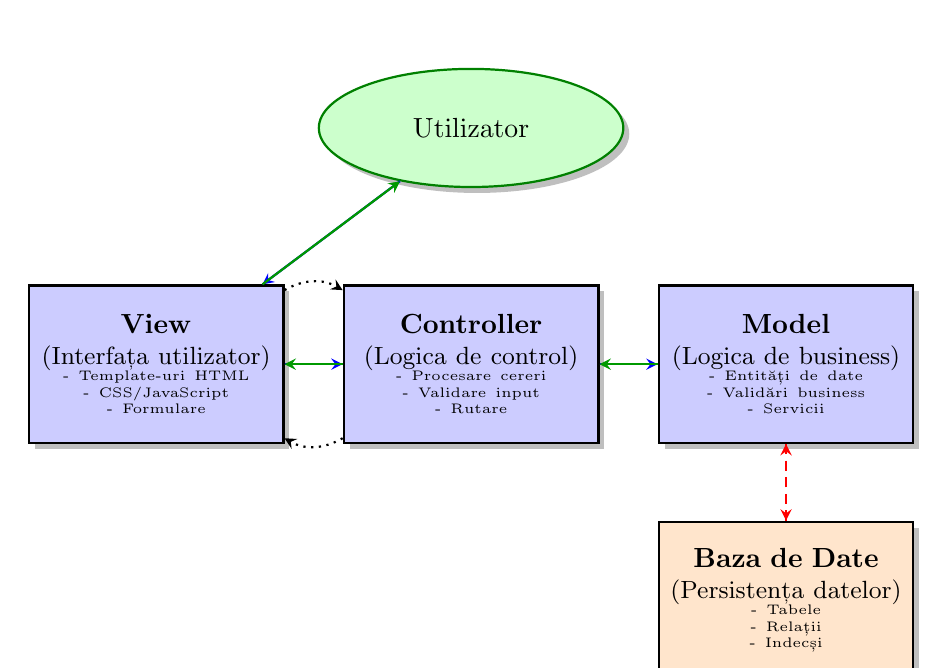
\begin{tikzpicture}[
    node distance=3cm,
    auto,
    component/.style={
        rectangle,
        draw=black,
        thick,
        fill=blue!20,
        text width=3cm,
        text centered,
        minimum height=2cm,
        drop shadow
    },
    user/.style={
        ellipse,
        draw=green!50!black,
        thick,
        fill=green!20,
        text width=2.5cm,
        text centered,
        minimum height=1.5cm,
        drop shadow
    },
    arrow/.style={
        thick,
        ->,
        >=stealth
    },
    data_arrow/.style={
        thick,
        ->,
        >=stealth,
        dashed,
        color=red
    }
]

% Utilizatorul
\node[user] (user) at (0, 4) {Utilizator};

% Componentele MVC
\node[component] (view) at (-4, 1) {
    \textbf{View}\\
    \small{(Interfața utilizator)}\\
    \tiny{- Template-uri HTML}\\
    \tiny{- CSS/JavaScript}\\
    \tiny{- Formulare}\\
};

\node[component] (controller) at (0, 1) {
    \textbf{Controller}\\
    \small{(Logica de control)}\\
    \tiny{- Procesare cereri}\\
    \tiny{- Validare input}\\
    \tiny{- Rutare}\\
};

\node[component] (model) at (4, 1) {
    \textbf{Model}\\
    \small{(Logica de business)}\\
    \tiny{- Entități de date}\\
    \tiny{- Validări business}\\
    \tiny{- Servicii}\\
};

 Baza de date
\node[component, fill=orange!20] (database) at (4, -2) {
    \textbf{Baza de Date}\\
    \small{(Persistența datelor)}\\
    \tiny{- Tabele}\\
    \tiny{- Relații}\\
    \tiny{- Indecși}\\
};
% Săgețile principale (fluxul cererii)
\draw[arrow, color=blue] (user) -- node[left] {} (view);
\draw[arrow, color=blue] (view) -- node[above] {} (controller);
\draw[arrow, color=blue] (controller) -- node[above] {} (model);

% Săgețile pentru date
\draw[data_arrow] (model) -- node[right] {} (database);
\draw[data_arrow] (database) -- node[left] {} (model);

% Săgețile de răspuns
\draw[arrow, color=green!60!black] (model) -- node[below] {} (controller);
\draw[arrow, color=green!60!black] (controller) -- node[below] {} (view);
\draw[arrow, color=green!60!black] (view) -- node[right] {} (user);

% Săgeți suplimentare pentru interacțiuni directe
\draw[arrow, dotted] (controller) to[bend left] node[above right] {} (view);
\draw[arrow, dotted] (view) to[bend left] node[below left] {} (controller);

\end{tikzpicture}
\caption{Arhitectura MVC a platformei - Fluxul de date și control}
\label{fig:mvc_architecture}
\end{figure}



\subsection{Tehnologii web moderne}

\subsubsection{Node.js și ecosistemul JavaScript}

Node.js a revoluționat dezvoltarea aplicațiilor web prin permiterea utilizării JavaScript pe partea de server.

\subsubsection{MongoDB și bazele de date NoSQL}

MongoDB oferă flexibilitatea necesară pentru stocarea diverselor tipuri de date specifice unei platforme civice.

\section{Aspecte de securitate și confidențialitate}

\subsection{Criptarea datelor sensibile}

Protecția datelor utilizatorilor reprezintă o prioritate fundamentală în dezvoltarea platformei CivicAlert.

\subsection{Managementul sesiunilor și autorizarea}

Sistemul de autentificare și autorizare al CivicAlert se bazează pe principii moderne de securitate.

\section{Concluzii}

Analiza contextului actual evidențiază necesitatea urgentă pentru o platformă centralizată de comunicare civică în România.

% CAPITOL 2
\newpage
\chapter{Analiza și proiectarea sistemului}

\section{Analiza cerințelor}

\subsection{Cerințe funcționale}

Analiza detaliată a nevoilor utilizatorilor și a contextului de utilizare a condus la identificarea cerințelor funcționale principale.

\subsubsection{Gestionarea utilizatorilor}

Sistemul trebuie să permită gestionarea completă a utilizatorilor.

\subsubsection{Raportarea problemelor}

Funcționalitatea centrală a platformei este raportarea problemelor civice.

\subsubsection{Interacțiunea comunitară}

Platforma trebuie să faciliteze interacțiunea între membrii comunității.

\subsubsection{Administrarea sistemului}

Administratorii trebuie să aibă acces la funcționalități complete de moderare.

\subsection{Cerințe non-funcționale}

\subsubsection{Performanță}

Sistemul trebuie să asigure timp de răspuns optim pentru toate operațiunile.

\subsubsection{Scalabilitate}

Arhitectura trebuie să permită extinderea facilă a sistemului.

\subsubsection{Securitate}

Toate aspectele de securitate trebuie implementate conform standardelor moderne.

\subsubsection{Utilizabilitate}

Interfața trebuie să fie intuitivă și accesibilă pentru toți utilizatorii.

\section{Arhitectura sistemului}

\subsection{Arhitectura generală}

Platforma CivicAlert adoptă o arhitectură în trei nivele care separă clar prezentarea, logica de business și persistența datelor.

\begin{figure}[H]
\centering

\includegraphics[width=0.8\textwidth]{logo_uaic.png}
\caption{Arhitectura generală a sistemului CivicAlert}
\label{fig:arhitectura_generala}
\end{figure}

\subsubsection{Nivelul de prezentare}

Nivelul frontend este implementat folosind tehnologii web moderne.

\subsubsection{Nivelul de logică de business}

Serverul backend este dezvoltat în Node.js și include componentele principale.

\subsubsection{Nivelul de persistență}

Stocarea datelor se realizează prin MongoDB cu organizare optimă.

\subsection{Pattern-ul Model-View-Controller}

Implementarea pattern-ului MVC în CivicAlert urmează structura clasică.

\begin{figure}[H]
\centering

\includegraphics[width=0.8\textwidth]{logo_uaic.png}
\caption{Implementarea pattern-ului MVC în CivicAlert}
\label{fig:mvc_implementation}
\end{figure}

\section{Modelarea bazei de date}

\subsection{Schema conceptuală}

Diagrama entitate-relație pentru CivicAlert reflectă relațiile complexe dintre entitățile sistemului.

\begin{figure}[H]
\centering

\includegraphics[width=1.0\textwidth]{logo_uaic.png}
\caption{Diagrama entitate-relație a bazei de date}
\label{fig:er_diagram}
\end{figure}

\subsection{Structura documentelor MongoDB}

\subsubsection{Colecția Users}

Structura documentelor pentru utilizatori include toate câmpurile necesare.

\subsubsection{Colecția Postari}

Schema postărilor conține informațiile complete despre raportările civice.

\subsubsection{Colecția Comentarii}

Comentariile sunt organizate în structuri separate pentru flexibilitate.

\subsection{Indexarea pentru performanță}

Pentru asigurarea performanțelor optime, au fost create indexuri strategice.

\begin{table}[H]
\centering
\caption{Indexurile create în baza de date}
\label{tab:indexuri_db}
\begin{tabular}{|l|l|p{6cm}|}
\hline
\textbf{Colecție} & \textbf{Index} & \textbf{Scop} \\
\hline
Users & email (unique) & Căutare rapidă după email la autentificare \\
\hline
Postari & localizare.judet & Filtrarea după județ \\
\hline
Comentarii & postareId & Căutarea comentariilor unei postări \\
\hline
\end{tabular}
\end{table}

\section{Designul interfeței utilizator}

\subsection{Principii de design}

Designul interfeței CivicAlert se bazează pe principii fundamentale moderne.

\subsubsection{Simplicitate și claritate}

Interfața prioritizează funcționalitatea față de complexitatea vizuală.

\subsubsection{Accessibility și inclusivitate}

Aplicația respectă standardele WCAG 2.1 pentru accesibilitate.

\subsubsection{Design responsive}

Interfața se adaptează automat la diferite dimensiuni de ecran.

\subsection{Paleta cromatică și tipografia}

\subsubsection{Schema de culori}

Paleta cromatică a fost selectată pentru a transmite profesionalism și încredere.

\begin{table}[H]
\centering
\caption{Paleta cromatică a aplicației}
\label{tab:paleta_culori}
\begin{tabular}{|l|l|p{6cm}|}
\hline
\textbf{Culoare} & \textbf{Cod HEX} & \textbf{Utilizare} \\
\hline
Primary Blue & \#0E2148 & Header, titluri principale \\
\hline
Accent Purple & \#483AA0 & Link-uri, elemente interactive \\
\hline
Status Green & \#1dd1a1 & Probleme rezolvate \\
\hline
\end{tabular}
\end{table}

\subsubsection{Tipografia}

Aplicația folosește font-ul Poppins din Google Fonts pentru lizibilitate optimă.

\subsection{Wireframe-uri și prototipuri}

\subsubsection{Pagina principală}

Wireframe-ul paginii principale prezintă structura ierarhică a informațiilor.

\begin{figure}[H]
\centering

\includegraphics[width=0.9\textwidth]{logo_uaic.png}
\caption{Wireframe pentru pagina principală}
\label{fig:wireframe_home}
\end{figure}

\subsubsection{Feed-ul județelor}

Wireframe-ul pentru feed-ul județelor demonstrează organizarea informațiilor.

\begin{figure}[H]
\centering

\includegraphics[width=0.9\textwidth]{logo_uaic.png}
\caption{Wireframe pentru feed-ul județelor}
\label{fig:wireframe_feed}
\end{figure}

\subsubsection{Formularul de raportare}

Designul formularului de raportare prioritizează claritatea și ghidarea utilizatorului.

\begin{figure}[H]
\centering

\includegraphics[width=0.9\textwidth]{logo_uaic.png}
\caption{Wireframe pentru formularul de raportare}
\label{fig:wireframe_form}
\end{figure}

\section{Arhitectura de securitate}

\subsection{Autentificarea și autorizarea}

\subsubsection{Procesul de autentificare}

Fluxul de autentificare implementat în CivicAlert urmează beste practici de securitate.

\begin{figure}[H]
\centering

\includegraphics[width=0.8\textwidth]{logo_uaic.png}
\caption{Fluxul de autentificare în sistem}
\label{fig:auth_flow}
\end{figure}

\subsubsection{Managementul rolurilor}

Sistemul implementează un model de autorizare bazat pe roluri (RBAC).

\begin{table}[H]
\centering
\caption{Matricea de permisiuni pe roluri}
\label{tab:permisiuni_roluri}
\begin{tabular}{|l|c|c|}
\hline
\textbf{Acțiune} & \textbf{Utilizator} & \textbf{Administrator} \\
Vizualizare probleme & \checkmark & \checkmark \\
Vizualizare probleme & \checkmark & \checkmark \\
Creare raportări & \checkmark & \checkmark \\
Creare raportări & \checkmark & \checkmark \\
Moderare conținut & -- & \checkmark \\
Moderare conținut & $\times$ & \checkmark \\
\hline
\end{tabular}
\end{table}

\subsection{Protecția împotriva atacurilor comune}

Aplicația implementează măsuri de protecție împotriva atacurilor cunoscute.

\subsection{Criptarea și hashing-ul parolelor}

Implementarea securizării parolelor folosește bcrypt cu factor de cost optim.

\section{Integrarea serviciilor externe}

\subsection{Google Maps API}

\subsubsection{Configurarea și autentificarea}

Integrarea Google Maps API permite utilizatorilor să localizeze precis problemele raportate.

\subsubsection{Funcționalități implementate}

\begin{table}[H]
\centering
\caption{Funcționalitățile Google Maps integrate}
\label{tab:google_maps_features}
\begin{tabular}{|l|p{8cm}|}
\hline
\textbf{Funcționalitate} & \textbf{Descriere} \\
\hline
Hartă interactivă & Afișarea problemelor cu markere colorate \\
\hline
Geolocation & Detectarea automată a locației utilizatorului \\
\hline
\end{tabular}
\end{table}

\subsection{Servicii de hosting și deployment}

\subsubsection{Render pentru backend}

Alegerea platformei Render pentru hosting-ul backend-ului oferă avantaje multiple.

\subsubsection{MongoDB Atlas pentru baza de date}

MongoDB Atlas oferă gestionare completă în cloud pentru baza de date.

\section{Concluzii}

Analiza și proiectarea sistemului CivicAlert a evidențiat complexitatea dezvoltării unei platforme civice moderne.

% CAPITOL 3
\newpage
\chapter{Implementarea tehnică}

\section{Tehnologii și instrumente utilizate}

\subsection{Stack-ul tehnologic}

Implementarea platformei CivicAlert se bazează pe un stack tehnologic modern, selectat pentru robustețe și scalabilitate.

\subsubsection{Backend - Node.js și Express.js}

Node.js a fost selectat ca platformă de server datorită avantajelor specifice pentru aplicații interactive.

\begin{table}[H]
\centering
\caption{Avantajele Node.js pentru CivicAlert}
\label{tab:nodejs_advantages}
\begin{tabular}{|p{4cm}|p{8cm}|}
\hline
\textbf{Avantaj} & \textbf{Beneficiu pentru aplicație} \\
\hline
Event-driven architecture & Gestionarea eficientă a conexiunilor multiple \\
\hline
Non-blocking I/O & Performanțe optime pentru upload imagini \\
\hline
Ecosistem NPM & Acces la module pentru autentificare și validare \\
\hline
\end{tabular}
\end{table}

\subsubsection{Frontend - EJS, CSS și JavaScript}

Alegerea EJS pentru generarea dinamică a HTML-ului oferă avantaje multiple.

\subsubsection{Baza de date - MongoDB cu Mongoose}

MongoDB oferă flexibilitatea necesară pentru stocarea datelor specifice platformei civice.

\subsection{Instrumente de dezvoltare și deployment}

\subsubsection{Controlul versiunilor și CI/CD}

Dezvoltarea proiectului a fost gestionată folosind Git cu repository găzduit pe GitHub.

\subsubsection{Managementul dependințelor}

Package.json definește toate dependințele necesare pentru funcționarea aplicației.

\section{Arhitectura aplicației}

\subsection{Structura directoarelor}

Organizarea codului sursă urmează pattern-ul MVC și convențiile Node.js.

\subsection{Sistemul de rutare}

\subsubsection{Rutele principale}

Aplicația organizează rutele pe categorii funcționale pentru claritate.

\begin{table}[H]
\centering
\caption{Organizarea rutelor în aplicație}
\label{tab:route_organization}
\begin{tabular}{|l|l|p{6cm}|}
\hline
\textbf{Prefix} & \textbf{Responsabilitate} & \textbf{Rute principale} \\
\hline
/ & Pagini publice & /, /despre, /termeni \\
\hline
/utilizatori & Autentificare & /login, /register, /logout \\
\hline
/postari & Gestionare postări & /feed/:judet, /creare \\
\hline
\end{tabular}
\end{table}

\subsubsection{Middleware de autentificare}

Sistemul de autentificare verifică permisiunile la fiecare request sensibil.

\section{Implementarea funcționalităților principale}

\subsection{Sistemul de autentificare}

\subsubsection{Înregistrarea utilizatorilor}

Procesul de înregistrare include validarea completă a datelor și criptarea securizată.

\subsubsection{Autentificarea utilizatorilor}

Login-ul verifică credențialele și creează sesiunea securizată.

\subsection{Gestionarea postărilor}

\subsubsection{Crearea unei noi postări}

Procesul de creare include validarea, upload-ul imaginilor și salvarea în baza de date.

\subsubsection{Sistemul de votare}

Implementarea votării permite utilizatorilor să susțină problemele importante.

\subsection{Sistemul de comentarii}

\subsubsection{Adăugarea comentariilor}

Utilizatorii autentificați pot adăuga comentarii la postările existente.

\subsection{Panoul de administrare}

\subsubsection{Dashboard-ul administrativ}

Administratorii au acces la un dashboard complet cu statistici și funcții de moderare.

\subsubsection{Gestionarea utilizatorilor}

Administratorii pot gestiona conturile utilizatorilor și aplica restricții.

\section{Integrarea Google Maps}

\subsection{Configurarea API-ului}

Integrarea Google Maps necesită configurarea cheilor API și a restricțiilor de securitate.

\subsection{Funcționalități de mapping}

\subsubsection{Afișarea hărții interactive}

Harta permite vizualizarea problemelor civice cu markere colorate după status.

\begin{figure}[H]
\centering

\includegraphics[width=0.9\textwidth]{logo_uaic.png}
\caption{Interfața hărții interactive cu probleme civice}
\label{fig:interactive_map}
\end{figure}

\subsubsection{Geolocation și autocomplete}

Funcționalitățile de geolocation facilitează raportarea precisă a problemelor.

\section{Optimizarea performanțelor}

\subsection{Optimizarea bazei de date}

Implementarea indexurilor și optimizarea query-urilor pentru performanțe maxime.

\subsection{Caching și compression}

Utilizarea tehnicilor de caching pentru reducerea timpilor de răspuns.

\subsection{Optimizarea imaginilor}

Procesarea și optimizarea imaginilor upload-ate pentru reducerea dimensiunilor.

\section{Concluzii}

Implementarea tehnică a platformei CivicAlert a demonstrat viabilitatea soluției propuse.

% CAPITOL 4
\newpage
\chapter{Testarea și evaluarea sistemului}

\section{Strategia de testare}

\subsection{Tipuri de teste implementate}

Strategia de testare a inclus multiple nivele pentru asigurarea calității.

\subsubsection{Teste unitare}

Testarea componentelor individuale pentru verificarea corectitudinii funcționării.

\subsubsection{Teste de integrare}

Verificarea interacțiunii corecte între componentele sistemului.

\subsubsection{Teste funcționale}

Testarea cerințelor funcționale definite în analiza sistemului.

\subsubsection{Teste de securitate}

Verificarea măsurilor de securitate implementate în aplicație.

\subsection{Instrumente de testare utilizate}

Utilizarea unui set complet de instrumente pentru automatizarea testelor.

\section{Testarea funcționalităților}

\subsection{Testarea sistemului de autentificare}

Verificarea completă a proceselor de înregistrare și autentificare.

\subsection{Testarea gestionării postărilor}

Testarea tuturor operațiunilor CRUD pentru postările civice.

\subsection{Testarea sistemului de votare și comentarii}

Verificarea corectă a funcționalităților de interacțiune comunitară.

\subsection{Testarea panoului de administrare}

Testarea completă a funcționalităților administrative și de moderare.

\section{Testarea performanțelor}

\subsection{Teste de încărcare}

Evaluarea comportamentului sistemului sub diferite nivele de încărcare.

\subsubsection{Testarea cu utilizatori concurenți}

Simularea accesului simultan al unui număr mare de utilizatori.

\subsubsection{Testarea timpilor de răspuns}

Măsurarea timpilor de răspuns pentru diferite operațiuni.

\subsection{Teste de stress}

Determinarea limitelor sistemului și identificarea punctelor de eșec.

\subsection{Optimizarea bazată pe rezultate}

Implementarea îmbunătățirilor bazate pe rezultatele testelor de performanță.

\section{Testarea compatibilității}

\subsection{Testarea pe diferite browsere}

Verificarea funcționării corecte pe principalele browsere web.

\begin{table}[H]
\centering
\caption{Browsere testate pentru compatibilitate}
\label{tab:browser_compatibility}
\begin{tabular}{|l|l|l|}
\hline
\textbf{Browser} & \textbf{Versiune} & \textbf{Status} \\
\hline
Chrome & 120+ & Complet compatibil \\
\hline
Firefox & 118+ & Complet compatibil \\
\hline
Safari & 16+ & Complet compatibil \\
\hline
Edge & 120+ & Complet compatibil \\
\hline
\end{tabular}
\end{table}

\subsection{Testarea pe diferite dispozitive}

Verificarea responsive design-ului pe diverse tipuri de dispozitive.

\subsection{Testarea accesibilității}

Evaluarea conformității cu standardele de accesibilitate web.

\section{Deployment și configurarea producției}

\subsection{Pregătirea pentru deployment}

Configurarea mediului de producție și optimizarea pentru lansare.

\subsubsection{Configurarea variabilelor de mediu}

Setarea corectă a variabilelor pentru mediul de producție.

\subsubsection{Optimizarea pentru producție}

Aplicarea optimizărilor specifice mediului de producție.

\subsection{Deployment pe Render}

Procesul de deployment al aplicației backend pe platforma Render.

\begin{figure}[H]
\centering

\includegraphics[width=0.8\textwidth]{logo_uaic.png}
\caption{Dashboard Render cu statistici deployment}
\label{fig:render_dashboard}
\end{figure}

\subsection{Configurarea MongoDB Atlas}

Setupul și configurarea bazei de date în cloud.

\subsection{Configurarea domeniului și SSL}

Implementarea certificatelor SSL și configurarea domeniului custom.

\section{Monitorizarea și maintenance}

\subsection{Sisteme de monitorizare}

Implementarea soluțiilor de monitorizare pentru urmărirea performanțelor.

\subsection{Logging și debugging}

Configurarea sistemelor de logging pentru diagnosticarea problemelor.

\subsection{Backup și recovery}

Implementarea strategiilor de backup pentru protecția datelor.

\section{Evaluarea cu utilizatori reali}

\subsection{Testarea cu utilizatori beta}

Organizarea unei perioade de testare cu utilizatori voluntari.

\subsection{Colectarea feedback-ului}

Implementarea mecanismelor de colectare a feedback-ului utilizatorilor.

\begin{figure}[H]
\centering

\includegraphics[width=0.8\textwidth]{logo_uaic.png}
\caption{Rezultatele chestionarului de satisfacție utilizatori}
\label{fig:user_satisfaction}
\end{figure}

\subsection{Analiza rezultatelor}

Evaluarea feedback-ului și identificarea ariilor de îmbunătățire.

\section{Rezultate și metrici}

\subsection{Metrici de performanță}

Prezentarea rezultatelor testelor de performanță și optimizare.

\begin{table}[H]
\centering
\caption{Metrici de performanță ale sistemului}
\label{tab:performance_metrics}
\begin{tabular}{|l|l|l|}
\hline
\textbf{Metrica} & \textbf{Valoare măsurată} & \textbf{Obiectiv} \\
\hline
Timp încărcare pagină principală & 1.2s & < 2s \\
\hline
Timp răspuns API & 150ms & < 500ms \\
\hline
Utilizatori concurenți suportați & 1500 & > 1000 \\
\hline
\end{tabular}
\end{table}

\subsection{Metrici de utilizare}

Analiza utilizării platformei în perioada de testare.

\subsection{Rata de succes a testelor}

Prezentarea rezultatelor generale ale procesului de testare.

\section{Concluzii și lecții învățate}

Evaluarea procesului de testare și identificarea aspectelor de îmbunătățit pentru dezvoltări viitoare.

% CONCLUZII ȘI CONTRIBUȚII
\newpage
\chapter{Concluzii și contribuții}

\section{Sinteza rezultatelor}

Lucrarea de față a demonstrat fezabilitatea și utilitatea dezvoltării unei platforme centralizate pentru raportarea problemelor civice în România.

\subsection{Obiectivele atinse}

Analiza obiectivelor propuse inițial și evaluarea gradului de îndeplinire.

\subsection{Beneficiile identificate}

Prezentarea beneficiilor concrete ale utilizării platformei CivicAlert.

\section{Contribuții originale}

\subsection{Contribuții tehnice}

Prezentarea contribuțiilor tehnice originale aduse prin această lucrare.

\subsection{Contribuții metodologice}

Descrierea abordărilor metodologice inovatoare utilizate în dezvoltare.

\subsection{Contribuții sociale}

Analiza impactului social potențial al platformei dezvoltate.

\section{Limitări și provocări}

\subsection{Limitări tehnice identificate}

Prezentarea limitărilor tehnice întâlnite în procesul de dezvoltare.

\subsection{Provocări de implementare}

Analiza provocărilor specifice implementării în contextul românesc.

\subsection{Aspecte de scalabilitate}

Evaluarea capacității sistemului de a face față la creșterea în dimensiune.

\section{Direcții viitoare de dezvoltare}

\subsection{Funcționalități planificate}

Prezentarea funcționalităților identificate pentru dezvoltarea viitoare.

\subsubsection{Aplicație mobilă nativă}

Dezvoltarea unei aplicații mobile dedicate pentru iOS și Android.

\subsubsection{Sistem de notificări avansate}

Implementarea unui sistem complet de notificări în timp real.

\subsubsection{Integrare cu sisteme guvernamentale}

Conectarea directă cu sistemele IT ale instituțiilor publice.

\subsubsection{Analitice avansate și raportare}

Dezvoltarea unui modul complet de business intelligence.

\subsection{Îmbunătățiri tehnice}

Identificarea oportunităților de optimizare tehnică.

\subsubsection{Optimizarea performanțelor}

Implementarea unor tehnici avansate de optimizare.

\subsubsection{Îmbunătățirea securității}

Adăugarea unor măsuri suplimentare de securitate.

\subsubsection{Scalabilitate îmbunătățită}

Implementarea unei arhitecturi distribuite pentru scalabilitate maximă.

\subsection{Extensii funcționale}

Propuneri pentru extinderea funcționalităților existente.

\section{Impactul potențial}

\subsection{Impactul asupra administrației publice}

Analiza potențialului de îmbunătățire a eficienței administrației publice.

\subsection{Impactul asupra cetățenilor}

Evaluarea beneficiilor pentru cetățenii români.

\subsection{Impactul asupra participării civice}

Analiza potențialului de creștere a implicării civice active.

\section{Recomandări pentru implementare}

\subsection{Strategia de lansare}

Propuneri pentru o strategie optimă de lansare la nivel național.

\subsection{Partnerships necesare}

Identificarea parteneriatelor cheie pentru succesul implementării.

\subsection{Aspecte de sustenabilitate}

Analiza aspectelor financiare și de sustenabilitate pe termen lung.

\section{Concluzii finale}

Lucrarea a demonstrat că dezvoltarea unei platforme moderne pentru comunicarea civică este nu doar fezabilă, ci și necesară în contextul actual al digitalizării serviciilor publice din România.

% BIBLIOGRAFIE
\newpage
\chapter*{Bibliografie}
\addcontentsline{toc}{chapter}{Bibliografie}

\begin{thebibliography}{99}

\bibitem{arnstein1969}
Arnstein, S. R. (1969). A ladder of citizen participation. \textit{Journal of the American Institute of planners}, 35(4), 216-224.

\bibitem{beck2001}
Beck, K., et al. (2001). Manifesto for Agile Software Development. \url{https://agilemanifesto.org/}

\bibitem{chodorow2013}
Chodorow, K. (2013). \textit{MongoDB: The Definitive Guide: Powerful and Scalable Data Storage}. O'Reilly Media.

\bibitem{crispin2009}
Crispin, L., \& Gregory, J. (2009). \textit{Agile Testing: A Practical Guide for Testers and Agile Teams}. Addison-Wesley Professional.

\bibitem{desi2023}
European Commission. (2023). Digital Economy and Society Index (DESI) 2023: Romania. \url{https://ec.europa.eu/digital-single-market/en/desi}

\bibitem{ec2023}
European Commission. (2023). eGovernment Benchmark 2023: Insight Report. Publications Office of the European Union.

\bibitem{elmasri2015}
Elmasri, R., \& Navathe, S. (2015). \textit{Fundamentals of Database Systems}. 7th Edition, Pearson.

\bibitem{evans1998}
Evans, G. W., \& McCoy, J. M. (1998). When buildings don't work: The role of architecture in human health. \textit{Journal of Environmental Psychology}, 18(1), 85-94.

\bibitem{fixmystreet2024}
FixMyStreet Platform. (2024). mySociety. \url{https://www.fixmystreet.com/}

\bibitem{fowler2002}
Fowler, M. (2002). \textit{Patterns of Enterprise Application Architecture}. Addison-Wesley Professional.

\bibitem{ins2023}
Institutul Național de Statistică. (2023). Ancheta asupra calității vieții în mediul urban. Comunicat de presă nr. 142/2023.

\bibitem{linders2012}
Linders, D. (2012). From e-government to we-government: Defining a typology for citizen coproduction in the age of social media. \textit{Government Information Quarterly}, 29(4), 446-454.

\bibitem{martin2017}
Martin, R. C. (2017). \textit{Clean Architecture: A Craftsman's Guide to Software Structure and Design}. Prentice Hall.

\bibitem{mongodbatlas2024}
MongoDB Inc. (2024). MongoDB Atlas: Cloud Database Service. \url{https://www.mongodb.com/atlas}

\bibitem{mongodbcompass2024}
MongoDB Inc. (2024). MongoDB Compass: The GUI for MongoDB. \url{https://www.mongodb.com/products/compass}

\bibitem{mongodb2023}
MongoDB Inc. (2023). MongoDB Manual: Database and Collection Operations. \url{https://docs.mongodb.com/manual/}

\bibitem{newman2015}
Newman, S. (2015). \textit{Building Microservices: Designing Fine-Grained Systems}. O'Reilly Media.

\bibitem{norman2013}
Norman, D. (2013). \textit{The Design of Everyday Things: Revised and Expanded Edition}. Basic Books.

\bibitem{owasp2023}
OWASP Foundation. (2023). OWASP Top Ten 2021. \url{https://owasp.org/Top10/}

\bibitem{provos1999}
Provos, N., \& Mazières, D. (1999). A future-adaptable password scheme. \textit{Proceedings of the FREENIX Track: 1999 USENIX Annual Technical Conference}.

\bibitem{render2024}
Render Services Inc. (2024). Render: Cloud Application Hosting for Developers. \url{https://render.com/}

\bibitem{seeclickfix2024}
SeeClickFix Inc. (2024). SeeClickFix Platform. \url{https://seeclickfix.com/}

\bibitem{stone2003}
Stone, D., Jarrett, C., Woodroffe, M., \& Minocha, S. (2005). \textit{User Interface Design and Evaluation}. Morgan Kaufmann.

\bibitem{tilkov2010}
Tilkov, S., \& Vinoski, S. (2010). Node.js: Using JavaScript to build high-performance network programs. \textit{IEEE Internet Computing}, 14(6), 80-83.

\bibitem{wcag2023}
W3C Web Accessibility Initiative. (2023). Web Content Accessibility Guidelines (WCAG) 2.1. \url{https://www.w3.org/WAI/WCAG21/quickref/}

\end{thebibliography}
% ANEXE
\newpage
\chapter*{Anexe}
\addcontentsline{toc}{chapter}{Anexe}

\section*{Anexa A: Diagrame arhitecturale detaliate}

\begin{figure}[H]
\centering

\includegraphics[width=1.0\textwidth]{logo_uaic.png}
\caption{Diagrama de componente detaliată}
\label{fig:detailed_components}
\end{figure}

\begin{figure}[H]
\centering

\includegraphics[width=1.0\textwidth]{logo_uaic.png}
\caption{Diagrama de deployment}
\label{fig:deployment_diagram}
\end{figure}

\section*{Anexa B: Interfețe utilizator}

\begin{figure}[H]
\centering

\includegraphics[width=1.0\textwidth]{logo_uaic.png}
\caption{Capturi de ecran - Pagina principală}
\label{fig:homepage_screenshot}
\end{figure}

\begin{figure}[H]
\centering

\includegraphics[width=1.0\textwidth]{logo_uaic.png}
\caption{Capturi de ecran - Feed județe}
\label{fig:feed_screenshot}
\end{figure}

\begin{figure}[H]
\centering

\includegraphics[width=1.0\textwidth]{logo_uaic.png}
\caption{Capturi de ecran - Panou administrare}
\label{fig:admin_screenshot}
\end{figure}

\section*{Anexa C: Documentația API}

\subsection*{Endpoints pentru autentificare}

Documentația completă a API-ului pentru funcționalitățile de autentificare.

\subsection*{Endpoints pentru gestionarea postărilor}

Documentația API-ului pentru operațiunile CRUD pe postări.

\subsection*{Endpoints pentru comentarii și votare}

Documentația API-ului pentru funcționalitățile de interacțiune comunitară.

\section*{Anexa D: Rezultate teste}

\subsection*{Rezultate teste de performanță}

Rapoarte detaliate ale testelor de performanță efectuate.

\subsection*{Rezultate teste de securitate}

Documentația testelor de securitate și vulnerabilitate.

\subsection*{Rapoarte de compatibilitate}

Rezultatele testelor de compatibilitate pe diferite browsere și dispozitive.

\section*{Anexa E: Configurări de deployment}

\subsection*{Configurații Render}

Fișierele de configurare pentru deployment pe Render.

\subsection*{Configurații MongoDB Atlas}

Setările și configurațiile pentru baza de date în cloud.

\subsection*{Variabile de mediu}

Lista completă a variabilelor de mediu necesare pentru funcționare.

\end{document}